%%% Research Diary - Entry
%%% Template by Mikhail Klassen, April 2013
%%% Modified by Pranav Sanghavi, May 2018
\documentclass[11pt,letterpaper]{article}

\newcommand{\workingDate}{\textsc{\today}}
\newcommand{\userName}{Pranav Sanghavi}
\usepackage{researchdiary_png}
\usepackage{circuitikz}


\title{jskfbadbf}


\begin{document}


{\Huge March 29 2018}\\[5mm]

\section*{Buckhannon RFI field test Memo}

\section{Set Up}

The Radio frequency test was conducted using a passive antenna clover (same design as HIRAX antennas). Amplification provided through p103 21dB amplifiers -- 2 amplifiers, each requiring a voltage of 5V. This voltage is supplied through a commercial battery pack. The voltage drawn from the battery is 5.57V. The signal chain (in Figure \ref{fig:signalchain}) is connected by a 1'  RG402 SMA cable between the antenna and the first p103 amplifier and a 10' LMR-195 SMA between the 3dB attenuator and the spectrometer. 

\begin{figure}[h]
\centering
\begin{circuitikz} 

\draw (0,0) node[antenna]{}	;
\draw (0,0) to[amp,t=p103,l_=$+21\,$dB] 	++(1.5,0);
\draw (1.5,0) to[amp,t=p103,l_=$+21\,$dB] 	++(1.5,0);
\draw (3,0) to[generic,l_=$-4\,$dB] 	++(1.5,0);
\draw (4.5,0) to[bandpass,l_=$400-800\,$MHz] 	++(3,0);
\draw (7.5,0) to[generic,l_=$-3\,$dB, -o] 	++(1.5,0) node[anchor=west]{Spectrometer};

\end{circuitikz}
\caption{Signal Chain for the RFI test. } \label{fig:signalchain}
\end{figure}

\section{Tests}

The the above set up was used to measure the environment signal levels at three locations: 1) the water tower, 2) the transmission tower and 3) Christopher Hall. The last location is of interest. In all three locations data was collected from the spectrometer. Power with the resolution resolution bandwidth of 10KHz between 0 and 3GHz was recorded. This was compared to the same set up in the lab with the antenna replaced by a  $50 \Omega$ terminal, this would provide us with a reference noise from an equivalent source at room temperature $\approx 300 \rm{K}$. As observed the data (plotted in Figure \ref{fig:signallevels}) the noise levels at the Christopher hall site falls below the in-lab $50 \Omega$ noise for $\approx 25\% $ of the bandwidth.


\begin{figure}
\centering
	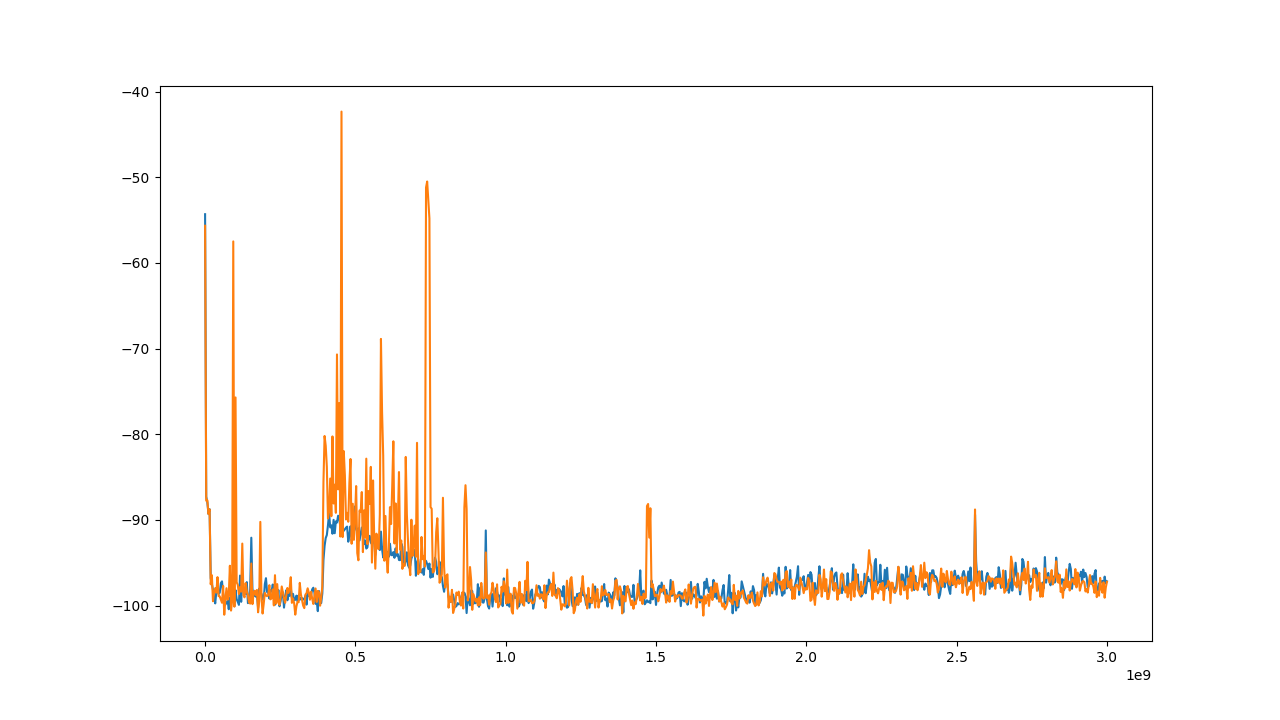
\includegraphics[width = \textwidth]{Figure_1-1}
	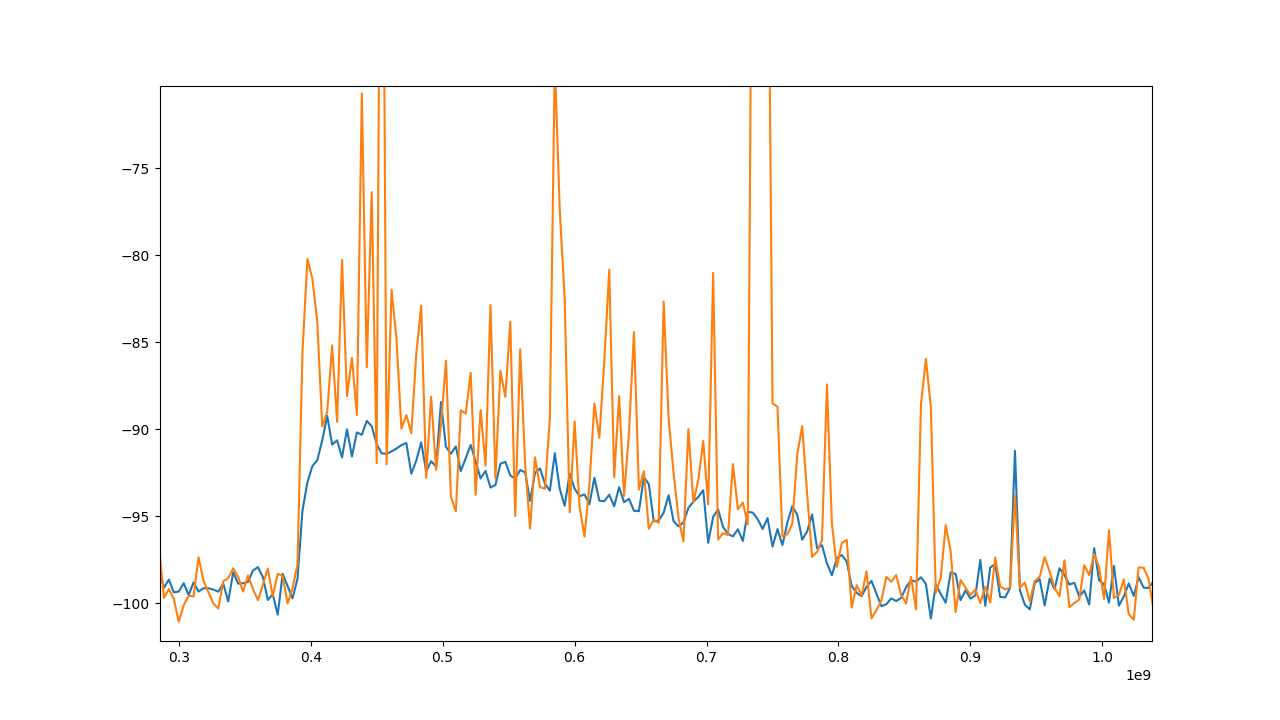
\includegraphics[width = \textwidth]{Figure_1-2}
	\caption{Signal Levels at Christopher Hall and in-lab. The Orange line is the signal from the site and the blue line is the signal chain with a $50 \Omega$ input in the lab corresponding to room temperature. The bottom figure us the zoomed in view of the bandwidth of interest.} \label{fig:signallevels}

\end{figure}


\end{document}